\documentclass[10pt,a4paper]{article}
\usepackage[utf8]{inputenc}
\usepackage[a4paper, margin=1.6cm, top=1.7cm, bottom=1.7cm]{geometry}
\usepackage{amsmath,amssymb}
\usepackage{xcolor}
\usepackage[most]{tcolorbox}
\usepackage{booktabs}
\usepackage{colortbl}
\usepackage{fancyhdr}
\usepackage{graphicx}
\usepackage{enumitem}

% Exact colors from original summary
\definecolor{themeblue}{rgb}{0.1686, 0.3529, 0.5294}   % #2B5A87
\definecolor{lightbg}{rgb}{0.9098, 0.9333, 0.9569}     % #E8EEF4
\definecolor{accentred}{rgb}{0.7843, 0.2706, 0.2275}   % #C8453A

% Header and Footer
\pagestyle{fancy}
\fancyhf{}
\fancyhead[L]{\textcolor{themeblue}{\small Lecture 2 --- Data exploration}}
\fancyhead[R]{\textcolor{themeblue}{\small Summary Sheet}}
\renewcommand{\headrulewidth}{0.5pt}
\renewcommand{\headrule}{\hbox to\headwidth{\color{themeblue}\leaders\hrule height \headrulewidth\hfill}}
\fancyfoot[C]{\thepage}

\begin{document}

% Title Block
\begin{center}
    {\LARGE\bfseries\color{themeblue} PCA}\\[3pt]
    {\small\itshape Summary sheet --- Deep Learning (S.-A. Berrani, ENSIA 2026--2027)}\\[3pt]
    \textcolor{themeblue}{\rule{\textwidth}{0.6pt}}
\end{center}

% Core Idea Box (Bulky notation bullets removed as requested)
\begin{tcolorbox}[
    colframe=themeblue,
    colback=lightbg,
    coltitle=white,
    fonttitle=\bfseries\sffamily,
    title={Core idea \& notation},
    arc=2mm,
    boxrule=0.6pt,
    left=8pt, right=8pt, top=6pt, bottom=6pt
]
\textbf{PCA} is a purely \textit{descriptive}, exploratory method (no probabilistic model assumed, normality not required) that handles any number of quantitative variables. It moves from $p$ variables to $q < p$ new variables while distorting reality as little as possible.
\end{tcolorbox}

\vspace{4pt}

% Section 1
\noindent{\Large\bfseries\color{themeblue} 1. Goal and principle}\\[4pt]
\textbf{Goal:} find the projection that \textbf{minimizes information loss}, i.e. the one that \textbf{maximizes the dispersion} of the projected data.\\
\textbf{Variance (dispersion):} mean squared distance between the points and their centroid $c$:
\[
V = \frac{1}{n} \sum_{i=1}^n d^2(x_i, c)
\]
\textbf{Property:} going from $p$ to $q < p$ necessarily loses dispersion. The idea is to lose as little as possible by choosing the projection axes well.\par\vspace{4pt}
\begin{tcolorbox}[
    colframe=accentred,
    colback=white,
    arc=1.5mm,
    boxrule=0.5pt,
    left=8pt, right=8pt, top=5pt, bottom=5pt
]
\textbf{Key principle of PCA.} Choose the projection (the axes) so as to \textit{maximize the dispersion} of the projected points.
\end{tcolorbox}

\vspace{6pt}

% Section 2: Algorithm & Mathematical Derivation
\noindent{\Large\bfseries\color{themeblue} 2. Algorithm \& Mathematical Derivation}\\[4pt]
Given a data matrix $X$ of size $n \times p$ ($n$ individuals/samples, $p$ quantitative variables):

\begin{enumerate}[leftmargin=18pt, itemsep=5pt, topsep=2pt]
    \item \textbf{Data Preprocessing: Centering (and Scaling / Normalization):}
    \begin{itemize}[leftmargin=12pt, itemsep=2pt]
        \item \textbf{Centering ($x_{ik} \leftarrow x_{ik} - \bar{x}_k$):} Subtract the column mean $\bar{x}_k = \frac{1}{n}\sum_{i=1}^n x_{ik}$ from every feature column.
        \textit{Geometric meaning:} shifts the center of mass (centroid $c$) to the origin $(0, \dots, 0)$ so the PCA axes pass directly through the data cloud rather than measuring distance from an arbitrary origin.
        \item \textbf{Scaling ($x_{ik} \leftarrow \frac{x_{ik} - \bar{x}_k}{\sigma_k}$):} Optional division by standard deviation $\sigma_k$, enforcing unit variance $\operatorname{Var}(X_k) = 1$. The covariance matrix then coincides with the correlation matrix $R$.
    \end{itemize}

    \vspace{2pt}
    \begin{center}
    \small
    \begin{tabular}{lll}
    \toprule
    \rowcolor{lightbg}
     & \textbf{Centering only} & \textbf{Centering + scaling} \\
    \midrule
    \textbf{Operation} & subtract the mean of each variable & also divide by the standard deviation \\
    \addlinespace[2pt]
    \textbf{Use when} & variables are \textit{homogeneous} (same unit, scale) & variables are \textit{heterogeneous} \\
    \bottomrule
    \end{tabular}
    \end{center}
    \vspace{2pt}

    \item \textbf{Projected Variance $\operatorname{Var}(U)$ as a Quadratic Form:}
    Project the centered data $X$ onto an unknown unit direction vector $v \in \mathbb{R}^p$ ($\|v\|_2 = 1 \iff v^T v = 1$) to obtain the 1D projected coordinates (scores):
    \[
    U = X v \quad (n \times 1)
    \]
    Because $X$ is centered ($\bar{x}_k = 0$), the projected scores automatically have zero mean ($\bar{u} = \frac{1}{n}\sum_{i=1}^n u_i = 0$). The statistical variance of $U$ therefore eliminates the mean subtraction and simplifies to a pure vector dot product:
    \[
    \operatorname{Var}(U) = \frac{1}{n} \sum_{i=1}^n (u_i - \bar{u})^2 = \frac{1}{n} \sum_{i=1}^n u_i^2 = \frac{1}{n} U^T U
    \]
    Substituting $U = X v$ and applying the transpose identity $(AB)^T = B^T A^T$:
    \[
    \operatorname{Var}(U) = \frac{1}{n} (X v)^T (X v) = v^T \left(\frac{1}{n} X^T X\right) v = v^T \mathbf{\Sigma} v
    \]
    Recognizing $\mathbf{\Sigma} = \frac{1}{n} X^T X$ (or $\frac{1}{n-1} X^T X$) as the sample covariance matrix, the variance along axis $v$ becomes a quadratic form: $\operatorname{Var}(U) = v^T \mathbf{\Sigma} v$.\\[3pt]
    \textit{Dual viewpoint (Eckart \& Young, 1936):} Maximizing projected variance is mathematically equivalent to minimizing the reconstruction error: $\min_{u, v} J(u, v) = \|X - u v^T\|_F^2$.

    \item \textbf{Variance Maximization via Eigenpairs (Why Eigenvectors?):}
    Our optimization problem is to find the unit direction $v$ maximizing preserved variance:
    \[
    \max_{v} \; v^T (\mathbf{\Sigma} v) \quad \text{subject to} \quad v^T v = 1
    \]
    \begin{itemize}[leftmargin=12pt, itemsep=2pt]
        \item \textbf{Why $v$ must be an eigenvector:} $\mathbf{\Sigma}$ is fixed by the data. The quadratic form $v^T (\mathbf{\Sigma} v)$ is the dot product between unit vector $v$ and the transformed vector $\mathbf{\Sigma} v$. For a fixed unit length, the dot product is maximized when both vectors point in the exact same direction (parallel, $\cos 0^\circ = 1$):
        \[
        \mathbf{\Sigma} v = \lambda v \qquad (\text{or } X^T X v = a v)
        \]
        This is the exact definition of an eigenvector $v$ and its corresponding eigenvalue $\lambda$ (or $a$).
        \item \textbf{Why the variance equals $\lambda$:} Substituting $\mathbf{\Sigma} v = \lambda v$ back into the variance formula:
        \[
        \operatorname{Var}(U) = v^T (\mathbf{\Sigma} v) = v^T (\lambda v) = \lambda (v^T v) = \lambda(1) = \lambda
        \]
        Thus, the eigenvalue $\lambda$ (or $a/n$) is identically the variance preserved along axis $v$. To maximize variance, we select the eigenvector with the largest eigenvalue $\lambda_1$.
    \end{itemize}

    \item \textbf{How to Compute Eigenvalues and Unit Eigenvectors:}
    To compute the eigenpairs $(\lambda_i, v_i)$ from the $p \times p$ symmetric covariance matrix $\mathbf{\Sigma}$ (or $X^T X$):
    \begin{itemize}[leftmargin=12pt, itemsep=3pt]
        \item \textbf{Step (a) --- Find Eigenvalues ($\lambda_i$):} Solve the characteristic equation:
        \[
        \det(\mathbf{\Sigma} - \lambda I) = 0 \qquad \text{(for $2 \times 2$: } \lambda^2 - \operatorname{Tr}(\mathbf{\Sigma})\lambda + \det(\mathbf{\Sigma}) = 0\text{)}
        \]
        Sort the resulting real, non-negative eigenvalues in descending order: $\lambda_1 \ge \lambda_2 \ge \dots \ge \lambda_p \ge 0$.
        \item \textbf{Step (b) --- Find Each Raw Eigenvector ($v_{\text{raw}}$):} For each eigenvalue $\lambda_i$, substitute it back into the homogeneous linear system:
        \[
        (\mathbf{\Sigma} - \lambda_i I) v_{\text{raw}} = 0
        \]
        \item \textbf{Step (c) --- Normalize to Unit Length ($\|v_i\|_2 = 1$):} Divide each raw eigenvector by its Euclidean norm to enforce the unit-length constraint $\sum_{k=1}^p v_{ik}^2 = 1$:
        \[
        v_i = \frac{v_{\text{raw}}}{\|v_{\text{raw}}\|_2} = \frac{v_{\text{raw}}}{\sqrt{v_{i1}^2 + v_{i2}^2 + \dots + v_{ip}^2}}
        \]
    \end{itemize}

    \item \textbf{Projection, Reconstruction, and Explained Variance:}
    \begin{itemize}[leftmargin=12pt, itemsep=2pt]
        \item \textbf{Projection Matrix ($V$):} Keep the top $q$ unit eigenvectors ($q < p$) as columns: $V = \begin{bmatrix} v_1 & v_2 & \dots & v_q \end{bmatrix} \in \mathbb{R}^{p \times q}$.
        \item \textbf{Projected Coordinates ($U$):} Transform centered data into the reduced $q$-dimensional space:
        \[
        U = X V \quad (n \times q) \qquad \text{entry by entry: } u_i^j = \langle x_i, v_j \rangle = \sum_{k=1}^p x_{ik} v_{jk}
        \]
        \item \textbf{Reconstruction:} The rank-$q$ reconstruction of the original data is $X' = U V^T \in \mathbb{R}^{n \times p}$.
        \item \textbf{Cumulative Explained Variance Ratio:} Total variance is conserved ($\sum_{i=1}^p \lambda_i = \operatorname{Tr}(\mathbf{\Sigma})$). The proportion of information retained by keeping $q$ components is:
        \[
        \text{Cumulative EVR}_q = \frac{\sum_{k=1}^q \lambda_k}{\sum_{i=1}^p \lambda_i} = \frac{\sum_{k=1}^q a_k}{\sum_{i=1}^p a_i} \ge s
        \]
    \end{itemize}
\end{enumerate}

\vspace{3pt}
\begin{tcolorbox}[
    colframe=accentred,
    colback=white,
    arc=1.5mm,
    boxrule=0.5pt,
    left=8pt, right=8pt, top=4pt, bottom=4pt
]
\textbf{\color{accentred}Outliers.} PCA is very sensitive to noise: a few outliers can artificially rotate principal axes and alter the number of components needed to reach the target explained variance.
\end{tcolorbox}

\newpage

% Section 3 (Old Section 4)
\noindent{\Large\bfseries\color{themeblue} 3. Worked example with $X, U, V$ (toy data, $n=4, p=2$)}\\[3pt]
\textbf{Setup:} four individuals, two variables, columns already centered (sums = 0) and of the same scale:
\[
X = \begin{pmatrix} 2 & 1 \\ 1 & 2 \\ -1 & -2 \\ -2 & -1 \end{pmatrix} \quad (4 \times 2)
\]
\begin{enumerate}[leftmargin=18pt, itemsep=2pt, topsep=1pt]
    \item \textbf{Center/reduce:} column means are $0 \Rightarrow$ nothing to subtract; same scale $\Rightarrow$ no scaling.
    \item \textbf{Covariance matrix:} $X^T X = \begin{pmatrix} 10 & 8 \\ 8 & 10 \end{pmatrix}$.
    \item \textbf{Eigen-decomposition:}
    \[
    \det(X^T X - a I) = (10 - a)^2 - 64 = 0 \implies a_1 = 18, \quad a_2 = 2
    \]
    Eigenvectors: $(X^TX - 18I)v_1 = 0 \implies v_1 = \frac{1}{\sqrt{2}}\begin{pmatrix} 1 \\ 1 \end{pmatrix}$; \quad
    $(X^TX - 2I)v_2 = 0 \implies v_2 = \frac{1}{\sqrt{2}}\begin{pmatrix} 1 \\ -1 \end{pmatrix}$.
    \item \textbf{Sort:} $(a_1, v_1) = \left(18, \frac{1}{\sqrt{2}}\begin{pmatrix}1\\1\end{pmatrix}\right)$, then $(a_2, v_2) = \left(2, \frac{1}{\sqrt{2}}\begin{pmatrix}1\\-1\end{pmatrix}\right)$.
    \item \textbf{Keep $q = 1$:} $V = v_1 = \frac{1}{\sqrt{2}}\begin{pmatrix} 1 \\ 1 \end{pmatrix}$ ($p \times q = 2 \times 1$).
    \item \textbf{Project:} $U = XV$ ($4 \times 1$); with all axes kept, $V = [v_1 \ v_2]$ and $U$ is $4 \times 2$:
    \[
    U = XV = \frac{1}{\sqrt{2}}\begin{pmatrix} 3 & 1 \\ 3 & -1 \\ -3 & 1 \\ -3 & -1 \end{pmatrix}, \qquad \text{e.g. } u_1^1 = \frac{2\cdot 1 + 1\cdot 1}{\sqrt{2}} = \frac{3}{\sqrt{2}} \approx 2.12
    \]
\end{enumerate}
\textbf{Result:} first column of $U$ ($= u^1$) is the $q = 1$ representation. Reconstruction with $q = 1$: $X' = u^1 v_1^T$ gives row 1 $= (1.5, 1.5)$ instead of $(2, 1)$; error $J = \|X - X'\|_F^2 = 4 \times 0.5 = 2 = a_2$ (the discarded eigenvalue). Explained variance: $\frac{18}{18+2} = \mathbf{90\%}$.

\vspace{4pt}

% Section 4 (Old Section 5)
\noindent{\Large\bfseries\color{themeblue} 4. Explained variance: choosing $q$}\\[3pt]
Choose the smallest $q$ such that the cumulative explained variance meets a chosen threshold $s$:
\[
\frac{\sum_{i=1}^q a_i}{\sum_{i=1}^p a_i} \ge s
\]
Since $a_i$ is the inertia of axis $i$, this represents the proportion of total information retained.
\begin{center}
\small
\begin{tabular}{lcccc}
\toprule
\rowcolor{lightbg}
\textbf{Axis} & 1 & 2 & 3 & 4 \\
\midrule
Eigenvalue $a_i$ (lecture, 4 grades) & 28.23 & 12.03 & 0.03 & 0.01 \\
Explained variance & 0.70 & 0.30 & 0.00 & 0.00 \\
Cumulative & 0.70 & 1.00 & 1.00 & 1.00 \\
\midrule
Toy example above & 18 & 2 & --- & --- \\
Explained / cumulative & 0.90 & 0.10 / 1.00 & --- & --- \\
\bottomrule
\end{tabular}
\end{center}
\vspace{-2pt}
\noindent In the lecture's grades example ($\sum a_i = 40.30$), $q = 2$ retains $\approx 100\%$ of the total information.

\vspace{4pt}

% Quick-reference checklist & Exam reflex
\noindent{\Large\bfseries\color{themeblue} 5. Quick-reference checklist}\par\vspace{3pt}
\begin{center}
\small
\begin{tabular}{lll}
\toprule
\rowcolor{lightbg}
\textbf{Check} & \textbf{Tool} & \textbf{Pass looks like} \\
\midrule
\textbf{Normalization} & centering (+ scaling if heterogeneous) & column means = 0 \\
\textbf{Axes} & eigenpairs $(a_i, v_i)$ of $X^T X$, $\|v_i\| = 1$ & sorted $a_1 \ge a_2 \ge \dots \ge 0$ \\
\textbf{Choice of $q$} & $\sum_{i \le q} a_i / \sum_{i \le p} a_i$ & above threshold $s$ \\
\textbf{Individuals} & $U = XV$ & similar points are close in the plane \\
\textbf{Variables} & $r(c^j, X^i)$, correlation circle & long arrows near the circle \\
\textbf{Outliers} & inspect the data first & no isolated points dominating axis 1 \\
\bottomrule
\end{tabular}
\end{center}

\vspace{1pt}
\begin{tcolorbox}[
    colframe=themeblue,
    colback=lightbg,
    arc=1.5mm,
    boxrule=0.5pt,
    left=8pt, right=8pt, top=3pt, bottom=3pt
]
\textbf{\color{themeblue}Exam reflex:} (1) Center (and scale) $X \rightarrow$ (2) Compute $X^T X \rightarrow$ (3) Find eigenpairs $(a_i, v_i)$, sort descending $\rightarrow$ (4) Pick $q$ with $\frac{\sum_{i \le q} a_i}{\sum_{i \le p} a_i} \ge s \rightarrow$ (5) Build $V = [v_1 \dots v_q]$, project $U = XV \rightarrow$ (6) Plot individuals in $U$, analyze variables via $r(c^j, X^i)$ on the correlation circle.
\end{tcolorbox}

\newpage

% Section 6 (Old Section 6)
\noindent{\Large\bfseries\color{themeblue} 6. Studying the variables: flip the table and use correlations}\\[4pt]
\textbf{Idea:} position yourself in a different space by transposing the data perspective. Each initial variable $X^i$ (column $i$ of $X$) and each principal component $c^j$ (column $j$ of $U$) is viewed as a vector in $\mathbb{R}^n$.\\[4pt]
\textbf{Goal:} analyze the linear correlation coefficients $r(c^j, X^i)$ between initial variables and principal components.

\begin{enumerate}[leftmargin=18pt, itemsep=3pt, topsep=2pt]
    \item \textbf{Compute principal components:} $U = XV$ (columns $c^j = u^j$).
    \item \textbf{Compute correlation for every variable $i$ and axis $j$:}
    \[
    r(c^j, X^i) = \frac{\sum_k u_k^j x_k^i}{\sqrt{\sum_k (u_k^j)^2}\sqrt{\sum_k (x_k^i)^2}} \qquad \text{(since columns are centered)}
    \]
    \item \textbf{Gather in a $p \times q$ table of correlations} (``variables-factors'').
    \item \textbf{Plot variable $X^i$ as point $\big(r(c^1, X^i), r(c^2, X^i)\big)$ inside the correlation circle.}
    \item \textbf{Interpretation:} arrows close to each other $\Rightarrow$ strong positive correlation ($\approx 1$); orthogonal arrows $\Rightarrow$ uncorrelated ($\approx 0$); opposite arrows $\Rightarrow$ negative correlation ($\approx -1$).
\end{enumerate}

\noindent\textcolor{accentred}{\textbf{Example (toy data):}} $x^1 = (2, 1, -1, -2)$, $x^2 = (1, 2, -2, -1)$, $u^1 = \frac{1}{\sqrt{2}}(3, 3, -3, -3)$, $u^2 = \frac{1}{\sqrt{2}}(1, -1, 1, -1)$:
\[
r(c^1, X^1) = \frac{18/\sqrt{2}}{\sqrt{18}\sqrt{10}} = \frac{3}{\sqrt{10}} \approx 0.95, \qquad r(c^2, X^1) = \frac{\sqrt{2}}{\sqrt{2}\sqrt{10}} = \frac{1}{\sqrt{10}} \approx 0.32
\]

\begin{center}
\small
\begin{tabular}{lcc}
\toprule
\rowcolor{lightbg}
\textbf{Variable} & $c^1$ (90\%) & $c^2$ (10\%) \\
\midrule
$X^1$ & 0.95 & 0.32 \\
$X^2$ & 0.95 & $-0.32$ \\
\bottomrule
\end{tabular}
\end{center}
\vspace{-2pt}
\noindent\textit{Shortcut:} since $X^T u^j = a_j v_j$, $r(c^j, X^i) = v_j^i \frac{\sqrt{a_j}}{\|x^i\|}$. Check: $0.95^2 + 0.32^2 = 1$ (length = 1 on the circle).

\vspace{6pt}
\begin{center}
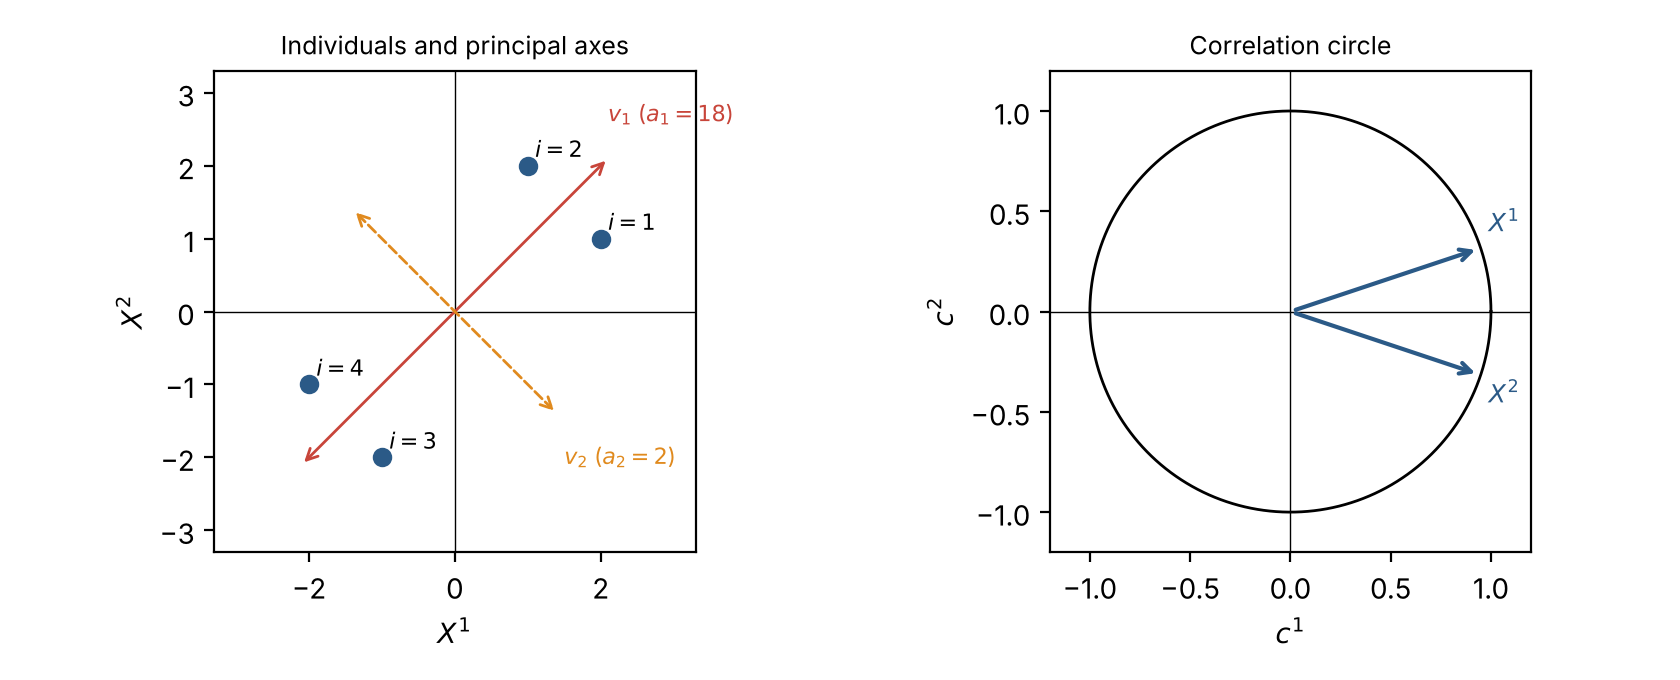
\includegraphics[width=0.88\textwidth]{pca_plots.png}\\[2pt]
{\footnotesize\textit{Left: individuals and principal axes $v_1, v_2$. Right: correlation circle, $X^1$ and $X^2$ are strongly correlated.}}
\end{center}

\vspace{4pt}
\begin{tcolorbox}[
    colframe=accentred,
    colback=white,
    arc=1.5mm,
    boxrule=0.5pt,
    left=8pt, right=8pt, top=5pt, bottom=5pt
]
\textbf{\color{accentred}Reading the circle.} Long arrows close to the circumference are well-represented by the retained axes; short arrows near the center are poorly represented and should not be interpreted.
\end{tcolorbox}

\end{document}
